\section{Higgs portal models}

\graphicspath{{1_TheoreticalBackground/Figures/HiggsPortal}}

The discovery of the Higgs boson by ATLAS and CMS experiments~\cite{Nisati:2015iwc} has paved the way for a new direction
in the searches for DM, in which one can explore the potential connections between the Higgs boson and the dark sector.
An interesting possibility is that the Higgs boson acting as a portal between the SM and dark sectors through
couplings to both sectors. There are both experimental and theoretical arguments that make this an interesting possibility.
Experimentally, the Higgs sector is far less explored and constrained, compared to the other sectors of the SM. Theoretically,
Higgs field is the only field that has a renormalizable
coupling to the dark sector, if DM is uncharged under the SM gauge group~\cite{Argyropoulos:2021sav}. Therefore, introducing 
DM Higgs-boson couplings is a well-motivated extension of the SM. Provided that the DM particles are not very heavy,
\textit{i.e.,} $m_{\textrm{DM}} < \frac{m_{\textrm{H}}}{2}$, such couplings would allow the Higgs boson to decay into DM particle
pairs, $\chi \bar{\chi}$. An example of this process is shown in Fig.~\ref{fig:vbfhinv_signal_diag}, where the SM Higgs boson
is produced via the vector boson fusion (VBF) process, and decays into $\chi\bar{\chi}$ final state.

\begin{figure}[htbp]
    \centering
    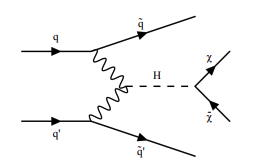
\includegraphics[width=0.4\textwidth]{vbf_signal_diagram.png}
    \caption{The VBF production of a SM-like Higgs boson, where the Higgs boson decays into a pair of DM particles, $\chi\bar{\chi}$.
    Diagram is taken from~\cite{VBFHinvAnalysisPaper}.}.
    \label{fig:vbfhinv_signal_diag}
\end{figure}

Given that the nature of the dark sector is mostly unknown, there are a multiple number of scenarios for the $H \chi \bar{\chi}$ coupling,
where the DM particle $\chi$ can be a scalar, a vector or a Majorana fermion~\cite{Djouadi:2011aa}. A brief overview of the 
theory of Higgs portal models under these different scenarios is provided in Sec.~\ref{subsec:higgs_portal_theory}, and the experimental
implications in particle colliders are discussed in Sec.~\ref{subsec:exp_signatures}.

\subsection{Theory}
\label{subsec:higgs_portal_theory}

This subsection aims to give a brief overview of the Higgs portal theories for different scenarios, following the footsteps of~\cite{Djouadi:2011aa}.
For the scenarios under which the DM particle is a scalar, vector or a Majorana fermion the corresponding Lagrangian terms are 

\begin{equation}
    \begin{split}
        \mathcal{L}_{S} &= -\frac{1}{2} m_{S}^{2} S^{2} - \frac{1}{4} \lambda_{S} S^{4} - \frac{1}{4} \lambda_{HSS} H^{\dag} H S^{2} \\
        \mathcal{L}_{V} &= -\frac{1}{2} m_{V}^{2} V_{\mu} V^{\mu} - \frac{1}{4} \lambda_{V} (V_{\mu} V^{\mu})^{2} + \frac{1}{4} \lambda_{HVV} H^{\dag} H V_{\mu} V^{\mu} \\
        \mathcal{L}_{f} &= -\frac{1}{2} m_{f} \bar{\chi} \chi - \frac{1}{4} \frac{\lambda_{Hff}}{\Lambda} H^{\dag} H \bar{\chi} \chi
    \end{split}
    \label{eq:higgs_portal_lagrangians}
\end{equation}
where the last terms represent the coupling between the DM-particle and SM-like Higgs boson, with $\lambda_{H\chi\bar{\chi}}$ being the coupling constants for each case.
It should be noted that the $H\chi\bar{\chi}$ coupling is not renormalizable in the fermionic case. The $S^{4}$ and $(V_{\mu} V^{\mu})^{2}$ are self-interaction terms
for scalar and vector DM particles, respectively. The first terms in each Lagrangian correspond to the mass term for the DM particle.

After electroweak symmetry breaking, the doublet field $H$ is written as $\phi(x) = \frac{1}{\sqrt{2}} \begin{pmatrix} 0, & v + h(x) \end{pmatrix}$ with $v = 246$ GeV
being the vacuum expectation value of the Higgs field. In that case, the physical masses of the DM particles can be written as~\cite{Djouadi:2011aa}

\begin{equation}
    \begin{split}
        M_{S}^2 &= m_{S}^2 + \frac{1}{2} \lambda_{hSS} v^{2} \\
        M_{V}^2 &= m_{V}^2 + \frac{1}{2} \lambda_{hVV} v^{2} \\
        M_{f}   &= m_{f}   + \frac{1}{2} \frac{\lambda_{hff}}{\Lambda} v^{2}
    \end{split}
\end{equation}

Provided that the DM particle $\chi$ is light enough for the $\textrm{H} \rightarrow \chi \bar{\chi}$ decay to occur (i.e. $M_{\chi} < M_{\textrm{H}} / 2$), there will be a non-zero
branching fraction for this decay of the Higgs boson, i.e. $B(\textrm{H} \rightarrow \chi \bar{\chi}) = \frac{\Gamma_{\chi\bar{\chi}}}{\Gamma_{\textrm{H}}} \neq 0$. The decay width for
$\textrm{H} \rightarrow \chi \bar{\chi}$ can be written as follows for the different scenarios being considered~\cite{Djouadi:2011aa}

\begin{equation}
    \begin{split}
        \Gamma_{\textrm{H} \rightarrow \textrm{SS}} &= \frac{\lambda_{hSS}^{2} v^{2} \beta_{S}}{64 \pi \mhiggs} \\
        \Gamma_{\textrm{H} \rightarrow \textrm{VV}} &= \frac{\lambda_{hVV}^{2} v^{2} \mhiggs^{3} \beta_{V}}{256 \pi M_{V}^{4}} \left( 1 - 4 \frac{M_V^2}{\mhiggs^2} + 12 \frac{M_V^4}{\mhiggs^4} \right) \\
        \Gamma_{\textrm{H} \rightarrow \textrm{ff}} &= \frac{\lambda_{hff}^{2} v^{2} \mhiggs \beta_{f}^{3}}{32 \pi \Lambda^{2}}
    \end{split}
\end{equation}
where $\beta_{X} = 1 - \sqrt{1 - 4 M_X^2 / \mhiggs^2}$. 
Therefore, observing these decays predicted by the Higgs portal models in particle colliders would be an important
leap towards understanding BSM physics. Observing these decays in particle colliders is the topic of the next subsection.

\subsection{Experimental signatures at colliders}
\label{subsec:exp_signatures}

Under the assumption of the DM particle ($\chi$) being a WIMP candidate, it is assumed that $\chi$ does not have electromagnetic interactions. That would imply
that in particle detectors like ATLAS and CMS, these particles would pass through without interacting with the detector components. Therefore, the event of a
$\textrm{H} \rightarrow \chi \bar{\chi}$ decay can be inferred by a large amount of transverse momentum imbalance in the event, \textit{i.e.,} large $p_T^{miss}$ (provided that there
is visible energy coming from other final state particles). Such decays are often referred to as ``invisible decays of the Higgs boson'', and very
commonly denoted as $\hinv$ This thesis will follow the same notation.

Such decays can be probed using proton-proton collisions by targeting events with the main production modes of the Higgs boson. Feynman diagrams for these production 
modes are shown in Fig.~\ref{fig:all_higgs_prod}. A very nice overview of all the production modes, 
together with their cross sections and kinematics are given in~\cite{Djouadi:2005gi}.

\begin{figure}
    \centering
    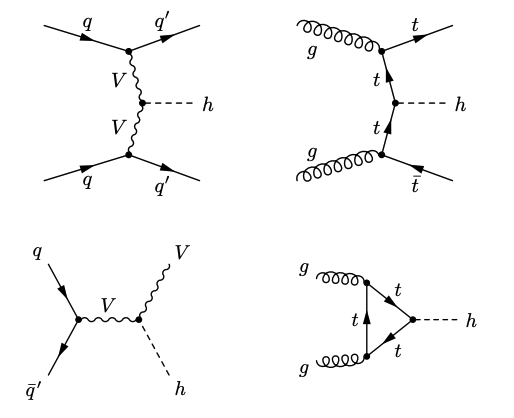
\includegraphics[width=0.7\textwidth]{all_higgs_prod.png}    
    \caption{Main production modes of the Higgs boson at a proton-proton collider. The production modes are vector boson fusion (top left), associated production with
    a pair of top quarks (top right), associated production with a vector boson (bottom left), and gluon-gluon fusion (bottom right). Diagrams are taken from~\cite{Argyropoulos:2021sav}.}
    \label{fig:all_higgs_prod}
\end{figure}

At the Large Hadron Collider (LHC), with a proton-proton collision center of mass energy of $\sqrt{s} = 13$ TeV, the dominating production mode is gluon-gluon fusion. Events from 
this production mode can be probed by targeting final states with an energetic hadronic jet\footnote{Hadronic jets arise from the hadronization of the
underlying final state quarks. Since individual quarks carry color charge, they cannot be observed individually due to the hypothesis of color confinement,
which arises from the gluon-gluon self interactions. On a mathematical basis, this is explained by the $g_{S} f^{ijk} G_{\mu}^{j} G_{\nu}^{k}$ terms appearing in 
Eq.~\ref{eq:gluon_field_strength}, which arise due to the non-commuting nature of SU(3) generators. Hence, jets are the corresponding 
experimental observables in particle colliders.} 
coming from initial state radiation, together with large $p_T^{miss}$ due to the invisible decay
of the Higgs boson. This is the so called ``monojet'' search. While there was no evidence observed for such events, this channel provided important constraints on the invisible
branching ratio of the Higgs boson, $B(\hinv) < 27.8\%$~\cite{CMS:2021far}. The associated production with a vector boson or a top-antitop quark pair have smaller cross sections,
but still are important final states to probe Higgs portal models~\cite{CMS:2023sdw}.

Search for $\hinv$ decays through the remaining production mode, vector boson fusion (VBF), is the topic of this thesis.
VBF has a lower production cross section, which is roughly an order of magnitude lower than the gluon-gluon fusion at $\sqrt{s} = 13$ TeV. But, it is still
a very sensitive channel in the searches of new physics. This is due to the uniqueness of the experimental signature of the final state, which is comprised of two energetic jets with large
spatial separation in the detector, and a large $p_T^{miss}$ because of the invisible decay of the Higgs boson. These two jets typically have small scattering angles with respect to the proton-proton
collision axis\footnote{A detailed explanation for this can be found in~\cite{Djouadi:2005gi}. It can be shown that the matrix element $\mathcal{M}$ is bounded by $1 / (p_T^2 + M_V^2)$,
where $p_T$ is the transverse momentum of the outgoing quarks, and $M_V$ is the mass of the vector boson. Hence, while the final state quarks are relatively energetic, the VBF cross-section is
suppressed for $p_{T} \gg M_{V}$, making the quarks (and hence the resulting final state jets from hadronization) more forward.}, 
making them forward in the detector and well-separated from each other. This unique final state signature of the VBF process can be used to reject a large amount of
SM backgrounds, making this channel very sensitive to signal. In fact, the previous searches done by collider experiments showed that VBF is the most sensitive channel, resulting
in the tightest constraints put on the $\brhinv$~\cite{CMS:2018yfx}. It is experimentally very motivating to continue the VBF $\hinv$ search with the new data coming in from
the Large Hadron Collider (LHC).

The rest of this thesis is structured as follows. Chapter~\ref{chap:apparatus} will give an overview of the experimental apparatus used to search for VBF $\hinv$ decays, namely the Large
Hadron Collider (LHC) and the Compact Muon Solenoid (CMS) detector. Chapter~\ref{chap:data_analysis} will then describe the analysis strategy, highlighting the analysis selections, the maximum
likelihood fit procedure and systematic uncertainties considered in the analysis. Chapter~\ref{chapter:results} will describe the results of the analysis and it's physics interpretations. Finally,
Chapter~\ref{chapter:outlook} will give perspective on the future direction of the CMS detector and the VBF $\hinv$ analysis, outlining upgrades on the detector and the triggering system, and
the search for new analysis methodologies using novel machine learning techniques.